\centerline{\large\bf APPENDIX B: Inductor Orientation Visualization}\label{appendix:orientation-visualization}
\addcontentsline{toc}{section}{Appendix B: Inductor Orientation Visualization}
Given an allowable board space defined as a prism, $P = \{\ell, w, h\}$, there are only three unique orientations for an air-core, solenoid-style inductor in the space. The inductor may be oriented with $A$ located on:
\begin{description}
\item[1.] the plane formed by $l$ and $w$ extending along $h$.
\item[2.] the plane formed by $l$ and $h$ extending along $w$.
\item[3.] the plane formed by $w$ and $h$ extending along $l$.
\end{description}

Figure \ref{fig:PossibleOrientations} depicts each of these orientations inside a prism with dimensions:

\begin{equation}\label{eq:PrismSimulation}
P = \{3, 2, 1\} \nonumber
\end{equation}

Notice the inductor consuming the most volume has its area $A$ on the plane formed by the two largest dimensions.

\begin{figure}[!htbp]
    \centering
    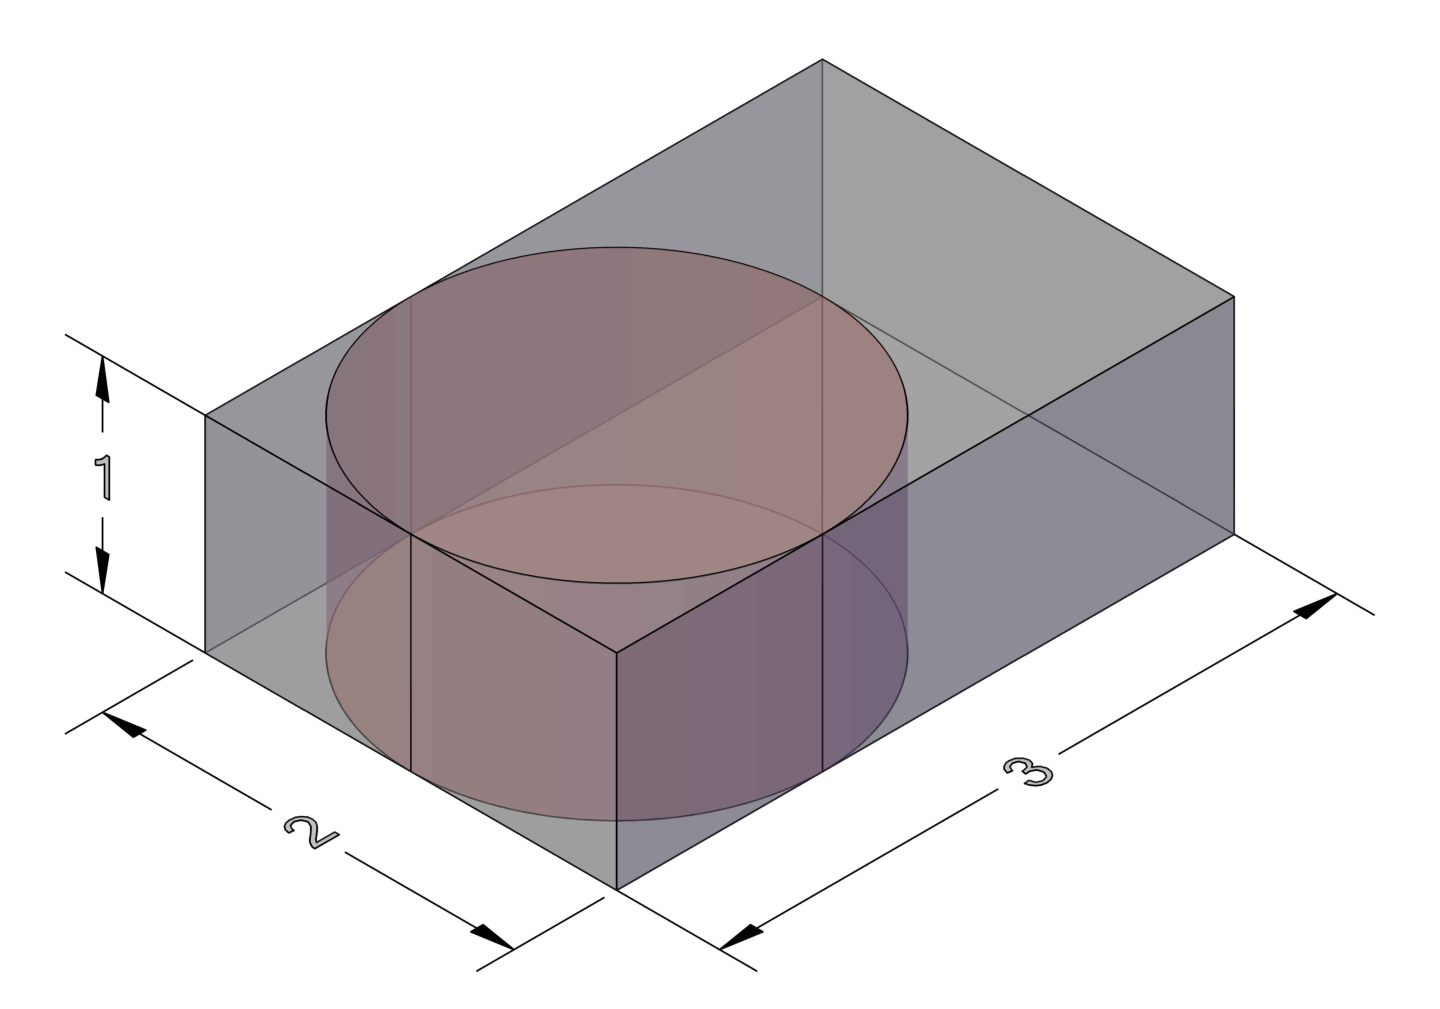
\includegraphics[width=0.30\linewidth]{fig/xyInductorCropped.pdf}
    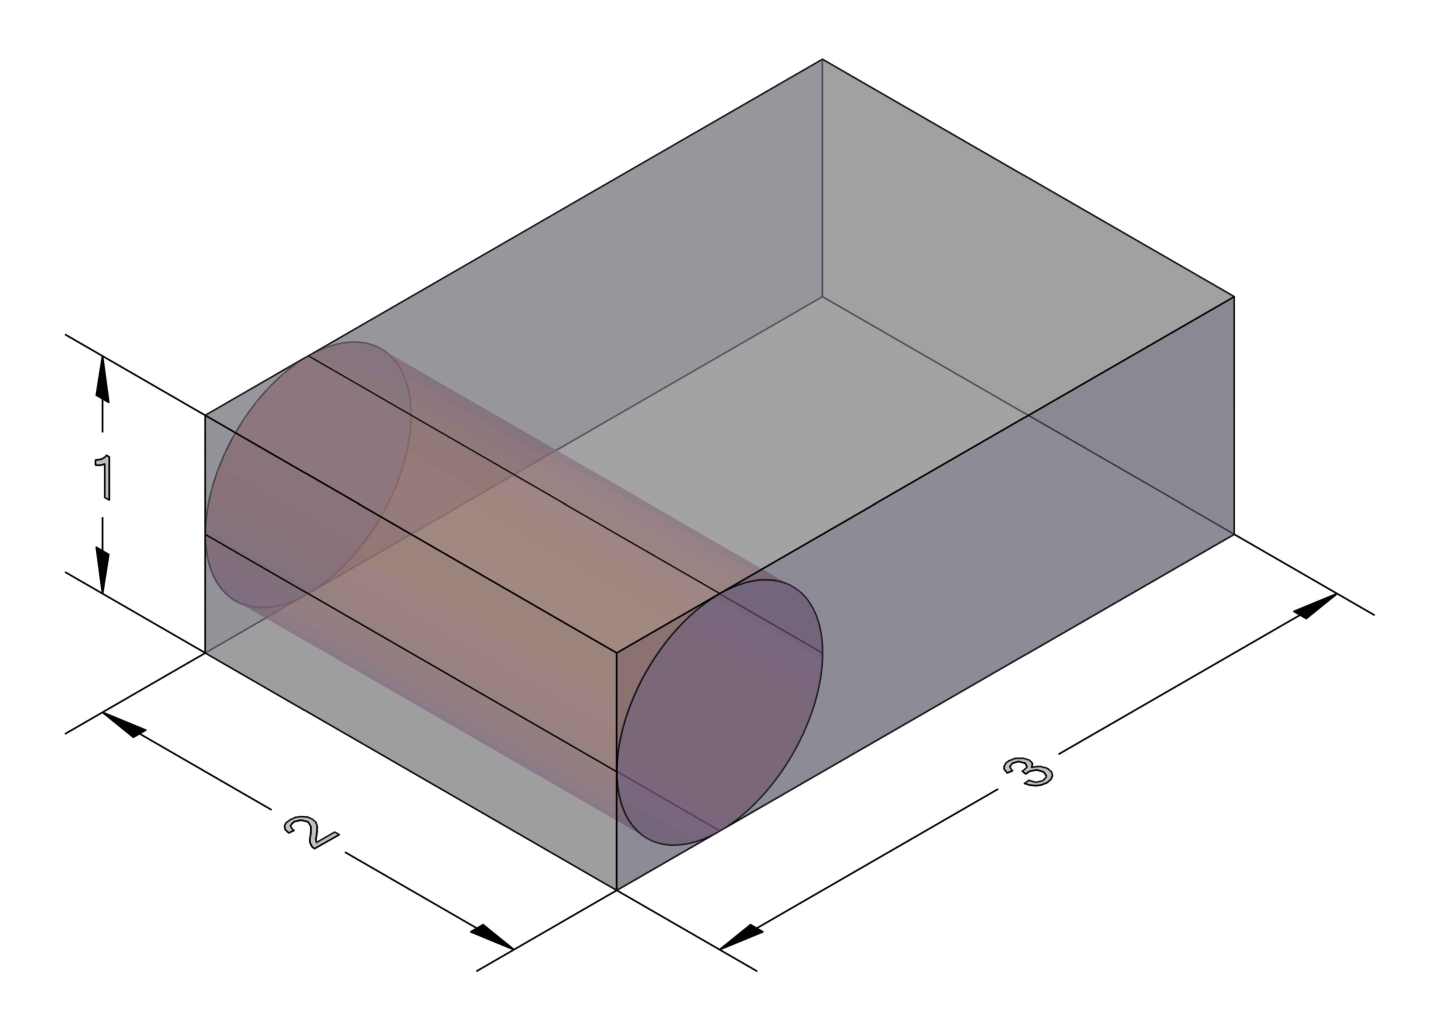
\includegraphics[width=0.30\linewidth]{fig/xzInductorCropped.pdf}
    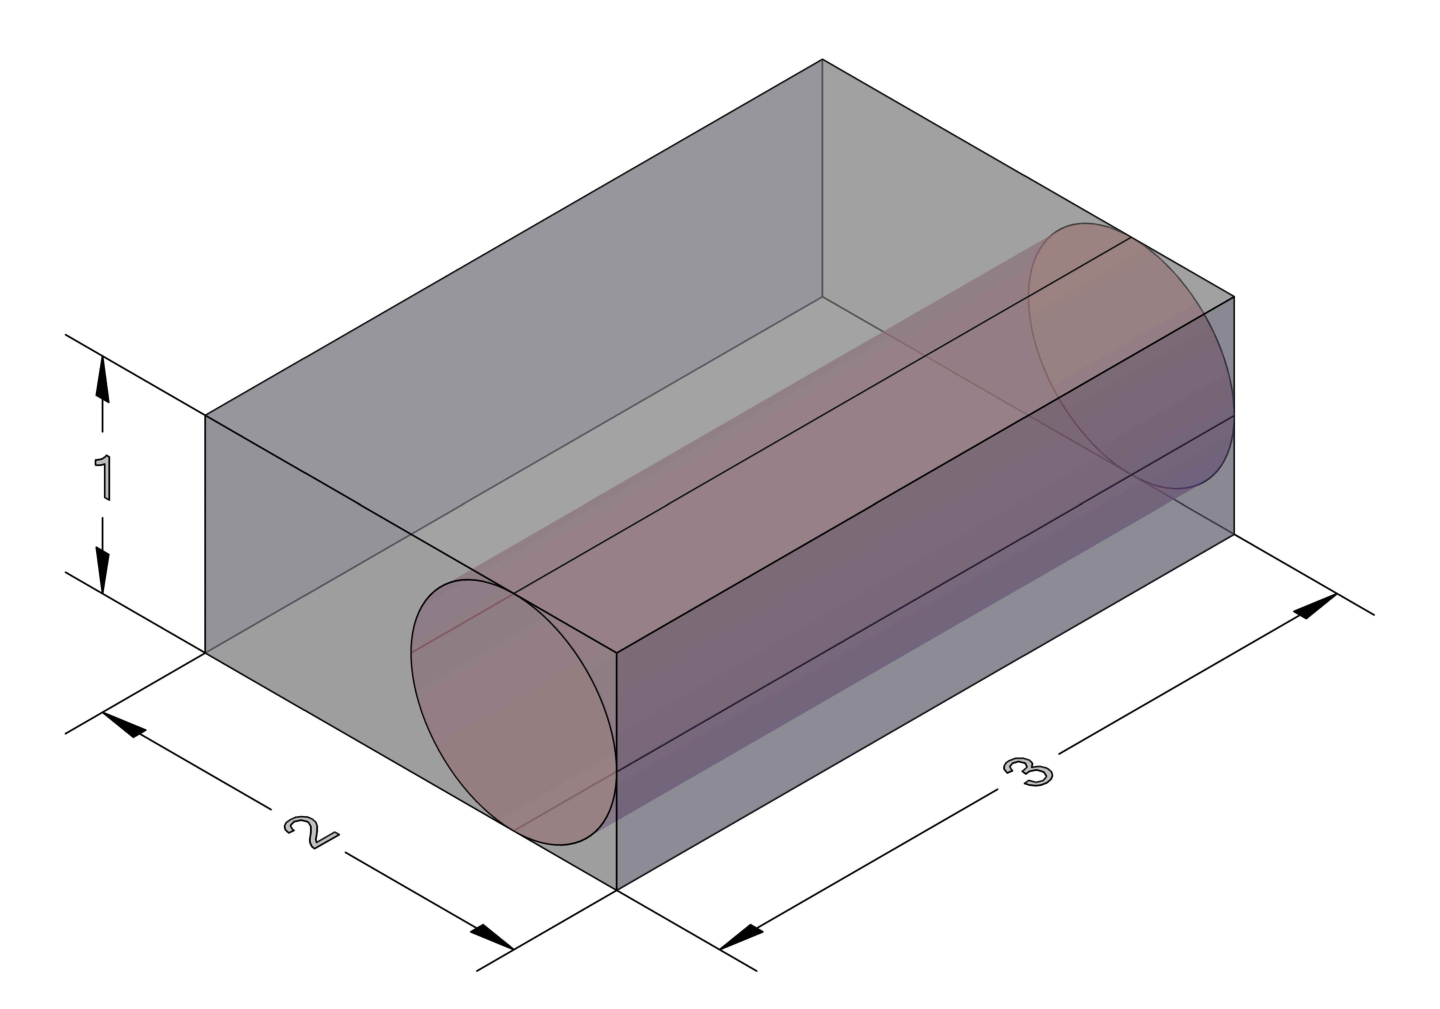
\includegraphics[width=0.30\linewidth]{fig/yzInductorCropped.pdf}
    \caption{Inductor Orientation Visualization}Possible orientations of air-core, solenoid-style inductors in a constrained space
    \label{fig:PossibleOrientations}
\end{figure}